\documentclass[hyperref={unicode=true}]{beamer}
\usepackage[utf8]{inputenc}
\usepackage[czech]{babel}
\usepackage[T1]{fontenc}
\usetheme{Malmoe}
\usecolortheme[named=brown]{structure}

\title{Hloubková automatická analýza angličtiny}
\subtitle{Diplomová práce}

\author[Ondřej Dušek]{Autor: Ondřej Dušek\\ Vedoucí práce: Prof. RNDr. Jan Hajič, Dr.}
\institute{Ústav formální a aplikované lingvistiky\\ MFF UK}
\date{6. září 2010}

\begin{document}

\begin{frame}
\titlepage
\end{frame}

\section{Úvod}

\begin{frame}{Úvod}

    \begin{block}{Automatická analýza významu}
    \begin{itemize}
        \item Popis významu závislostními stromy vs. propozicemi
        \item Identifikace propozic: 
        \begin{itemize}
            \item Identifikace a disambiguace predikátů
            \item Identifikace a klasifikace argumentů  
        \end{itemize}
        \item Použití strojového učení 
    \end{itemize}
    \end{block}    

    \begin{block}{Cíl práce} 
    Navhrnout a implementovat systém pro automatickou sémantickou analýzu v angličtině, otestovat na existujících datech (CoNLL~2009).
    \end{block}     

\end{frame}

\begin{frame}{Použitá data}
    \begin{block}{CoNLL 2009 Shared Task}
    \begin{itemize}
        \item Data pro 7 jazyků, vč. angličtiny, v jednotném formátu
        \item Disambiguace predikátů, identifikace a klasifikace argumentů 
        \item Jednotná evaluace
        \item Popisy soutěžních systémů a výsledná data jsou zveřejněná
    \end{itemize}
    \end{block}
    \begin{block}{Anglický korpus}
    \begin{itemize}
        \item Penn Treebank -- morfologická a syntaktická anotace
        \item PropBank / NomBank -- sémantické propozice pro slovesa a~substantiva   
    \end{itemize}
    \end{block}
\end{frame}

\begin{frame}{Sémantické značkování dat CoNLL 2009 -- příklad}
    \begin{columns}
    \begin{column}{0.6\textwidth}
    \begin{block}{Disambiguace predikátů}
    \begin{itemize}\scriptsize\setlength{\itemindent}{1em}
        \item[run.01] operate, procede \textit{(John runs the company.)}
        \item[run.02] walk quickly \\ \textit{(John ran the Boston Marathon.)}
        \item[run.03] cost \textit{(This watch runs \$30.)}
        \item[run.04] range, extend \\ \textit{(Shelves ran from floor to ceiling.)}
    \end{itemize}
    \end{block}
    \begin{block}{Identifikace a klasifikace argumentů}
    \scriptsize "`run.01"' -- valenční argumenty:
    \begin{itemize}\scriptsize
      \item[A0] operator
      \item[A1] machine, operation, procedure
      \item[A2] employer
      \item[A3] coworker
      \item[A4] instrumental
      \item[...] 
    \end{itemize}
    \end{block}
    \end{column}
    \begin{column}{0.4\textwidth}
    \begin{center}
    \scriptsize
    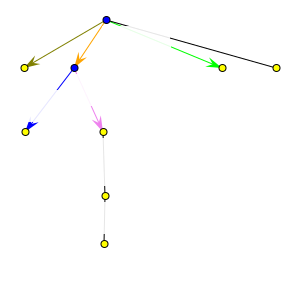
\includegraphics[width=\textwidth]{example-sentence} \\
    And their suspicions of each other run deep.
    \end{center}
    \end{column}
    \end{columns}
\end{frame}

\section{Implementace}

\begin{frame}{Běhové prostředí pro experimenty}
    \begin{block}{Cíle}
    \begin{itemize}
        \item Snadná konfigurovatelnost
        \item Dávkové zpracování úkolů, závislosti
        \item Paralelní provádění experimentů
    \end{itemize}
    \end{block}
    \begin{block}{Implementace}
    \begin{itemize}
        \item Integrace existujících nástrojů (WEKA, LP\_Solve)
        \item Modularita (obecný interface a nezávislost jednotlivých úkolů)
        \item Dávkové zpracování -- expanze úkolů 
        \begin{itemize}\item Wildcards, kombinace pouze odpovídajících si souborů \end{itemize}
    \end{itemize}
    \end{block}          
\end{frame}

\begin{frame}{Základní techniky (1)}
    \begin{block}{Klasifikátory}
    \begin{itemize}
        \item Logistická regrese
        \item Support Vector Machine 
    \end{itemize}
    \end{block}

    \begin{block}{Konverze dat}
    \begin{itemize}
        \item "`Zploštení"' formátu -- rozdělení lemmat / predikátů
        \begin{itemize}\item Zvětšení objemu dat\end{itemize}
        \item Rysy z anotace + generované rysy
        \item Filtrování
        \item Výběr rysů
        \begin{itemize}
            \item Hodnocení rysů (6 kritérií) a lineární přidávání
            \item Hladový algoritmus
        \end{itemize}
    \end{itemize}
    \end{block}
\end{frame}

\begin{frame}{Základní techniky (2)}
    \begin{block}{Generované rysy}
    \begin{itemize}
        \item Implementace dříve popsaných rysů
        \begin{itemize}
            \item Syntaktické -- sourozenci, děti, rodič
            \item Morfologické, topologické
        \end{itemize}
        \item Nové rysy
        \begin{itemize}
            \item \emph{Children Types} -- děti v závislosti na morfologii
            \item \emph{Clusters} -- sémantický clustering, implicitní informace (syntakticky / morfologicky vztažené k danému slovu)
        \end{itemize}
    \end{itemize}
    \end{block}

    \begin{block}{Evaluace}
    \begin{itemize}
        \item Využití existující evaluace CoNLL 2009
        \item Experimenty: standardní metriky, bootstrapový test
    \end{itemize}
    \end{block}
\end{frame}

\begin{frame}{Implementace systému}
    \begin{block}{Disambiguace predikátů}
    \begin{itemize}
        \item Rozdělení dat podle lemmat (nezávislé významy)
        \item Různé techniky vyběru rysů podle počtu významů lemmatu (kompromis rychlosti výpočtu a kvality výsledku)
    \end{itemize}
    \end{block}

    \begin{block}{Klasifikace argumentů}
    \begin{itemize}
        \item Spojení identifikace a klasifikace argumentů
        \item Oddělení klasifikace pro valenční argumenty / adverbiální doplnění
        \item "`Post-Inference"' -- unikátnost valenčních argumentů (dvě varianty)
    \end{itemize}
    \end{block}
\end{frame}

\section{Výsledky}

\begin{frame}{Výsledky systému na datech CoNLL 2009}
    \begin{block}{Celkové výsledky}
    \begin{tabular}{lcl}
        Disambiguace predikátů & 95.06 \% & accuracy \\
        Klasifikace argumentů &  64.42 \% & labeled $F_1$ \\
        Celkem & 75.00 \% & labeled $F_1$ \\ 
    \end{tabular}
    
    Pro přímočarý algoritmus post-inference.
    \end{block}
    
    \begin{block}{Srovnání s ostatními systémy ze soutěže CoNLL 2009}
    \begin{itemize}
        \item Celkový výsledek -- 15./21        
        \item Velmi dobrá disambiguace predikátů (4.)
        \item Průměrná kvalita klasifikace argumentů        
    \end{itemize}
    \end{block}
\end{frame}

\begin{frame}{Analýza výsledků}

    \begin{block}{Podrobný pohled}
    \begin{itemize}
        \item Disambiguace predikátů -- \emph{Children Types} i \emph{Clusters} často vybírané
        \item Klasifikace argumentů -- precision vs. recall
        \item Problém s adverbiálními doplněními u substantiv  
    \end{itemize}
    \end{block}

    \begin{block}{Možná zlepšení}
    \begin{itemize}
        \item Další generované rysy
        \item Podrobnější filtrování / výběr rysů
        \item Oddělení klasifikace adverbiálních doplnění pro substantiva a slovesa
        \item Speciální řešení koreferencí  
    \end{itemize}
    \end{block}
\end{frame}

\begin{frame}{Následný experiment: Aplikace na češtinu}
    \begin{itemize}
        \item Data pro češtinu z PDT 2.0
        \begin{itemize}\item Větší objem dat -- další slovní druhy, více významů\end{itemize}
        \item Úpravy pro jiné značení lemmat a významů predikátů  
        \item Úprava pro složitější morfologické značky
        \item Nutné úpravy generovaných rysů -- na základě morfologie
        \item Predicate disambiguation: 94.89 \% accuracy
    \end{itemize}    
\end{frame}

\end{document}

